\documentclass[a4paper,12pt]{article}
\usepackage{amsmath}
\usepackage{amssymb}
\usepackage{tikz}
\newcommand{\CommaPunct}{\mathpunct{\raisebox{0.5ex}{,}}}
\begin{document}
\title{ECE108 Assignment3} \author{Yi Fan Yu yf3yu@edu.uwaterloo.ca} \date{\today}

\maketitle

\pagenumbering{arabic}
\tableofcontents
\newpage
\renewcommand\thesubsection{\alph{subsection}}
\section{Rolling Dice}
\subsection{Dicerolling1,2,3,4,5,6}
How many times will the sequence 1,2,3,4,5,6 occur?  What is the
probability of this occurring?\\
\bigskip\\
well if $n \leq 6$, there is 0 chance of any sequence occuring\\
if $n = 6$, there is 1 occurence which means $\frac{1}{6^{6}}$ chance\\
if $n \geq 6$,there are 
  \[(n-5)!*6^{n-6}\text{occurences}\]
  which leads to a probability of occurence to
  \[\frac{(n-5)!*6^{n-6}}{6^{n}}\]

\subsection{DicerollingA,B,C}
How many times will the sum of the number of 1's and 2's equal the
sum of the number of 3's, 4's, 5's and 6's?  What is the probability
of this occurring?
let's say\\
\[ 1 \& 2 \mapsto A\]
\[ 3 \& 4 \mapsto B\]
\[ 5 \& 6 \mapsto C\]
$A \& B \& C$ with all equal possibilities of showing up (1/3)\\
Then we can say we are only throwing a 3 sided dice, therefore the total amount of possibilities while throwing is\\
\[3^n\]
using the analogy of undistinguishable $A$s and $ B\& C$s
our equation for $ \|A\|= \|B\|+\|C\|$
is \\
  \[ \frac{n!}{\frac{n}{3}! * \frac{2n}{3}!}\]
  \[ \frac {\frac{n!}{\frac{n}{3}! * \frac{2n}{3}!}} {3^{n}}\]
\subsection{DicerollingA,B,C Part2}
How many times will the sum of the number of 1's and 2's equal the
sum of the number of 3's and 4's and equal the sum of the number of
5's and 6's?  What is the probability of this occurring?\\
Same thing as part I, but now $A$s are indisguishable from $B$s and from $C$s. Therefore,
  \[\frac{n!}{\frac{n}{3}*!\frac{n}{3}!*\frac{n}{3}!}\]
  with the total probability at :\\
  \[ \frac {\frac{n!}{\frac{n}{3}*!\frac{n}{3}!*\frac{n}{3}!}} {3^{n}}\]
\subsection{Rolling 1s}
How many times will you roll a 1 twice in succession?  For the
purpose of this calculation, the sequence ...11.... counts as once,
but so does ...111....  The sequence ...1111... counts as twice.  What
is the probability of this occurring?

\subsection{Rolling 1s}
How many times will you roll a 1 twice in succession?  For the
How many times will you roll a 1 $k$-times in succession?  As with
the previous case, when a 1 is counted as part of a $k$-sequence, it
is not counted as part of a subsequent $k$-sequence.  What
is the probability of this occurring?

\subsection{Communication}
How many times will you roll a 1 twice in succession?  For the
You have a communications system that transmits bundles of data
from a source to a destination.  Most bundles are received correctly.
However, there is a random chance of the data in a bundle being in
error.  Roughly every $E^{th}$ bundle is in error.  If you transmit
$n$ bundles, what is the probability of two bundles in sequence being
in error?  what is the probability of $k$ bundles in sequence being in
error?

\section{Binomial Theorem}
Prove (using induction) the binomial theorem:
\[
(x+a)^n = \sum_{r=0}^n C(n‚ r)x^{n-r}a^r
\]
\subsection{Base Case}
n = 1 case:\\
\[(x+a) = \sum_{r=0}^1 C(n‚ r)x^{n-r}a^r\]
\[(x+a) = \binom{1}{0} x^{1} + \binom{1}{1}  a^1\]
\[(x+a) = x+a \blacksquare \]
\subsection{N+1 Case}
Assuming:
\[
(x+a)^n = \sum_{r=0}^n C(n‚ r)x^{n-r}a^r
\]
Show:
\[(x+a)^{n+1} = \sum_{r=0}^{n+1} C((n+1)‚ r)x^{(n+1)-r}a^r\]
Proof:
\[(x+a)^{n+1} = \sum_{r=0}^{n+1} C((n+1)‚ r)x^{(n+1)-r}a^r\]
\[(x+a)^{n+1} = (\sum_{r=0}^{n} C((n+1)‚ r)x^{(n+1)-r}a^r) \]

\section{Graph Questions}

\subsection{a graph with 5 vertices and 3 edges}
yes, any graph can exist with any amount of vertices and edges provided the number of edges are not bigger than the maximum possible amount.\\
for 5 vertices, the maximum amount of edges 
  \[\binom{5}{2} = 10\]
\begin{center}
  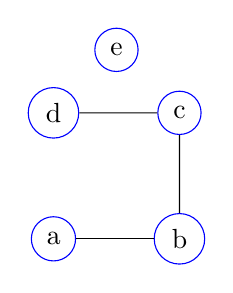
\begin{tikzpicture}
    [scale = .8, auto=center, every node/.style = {circle,draw = blue}]
    \node (n1) at (0,0) {a};
    \node (n2) at (2,0) {b};
    \node (n3) at (2,2) {c};
    \node (n4) at (0,2) {d};
    \node (n5) at (1,3) {e};

    \foreach \from/ \to in {n1/n2,n2/n3,n3/n4}
      \draw (\from) -- (\to);
  \end{tikzpicture}
\end{center}
    
\subsection{a graph with 5 odd-degree vertices with 3 edges}
  it is quite clear that with 3 edges, we are thinking of vertices with
  degree = 1.\\
\begin{center}
  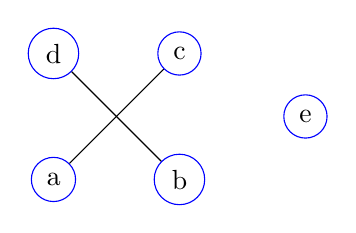
\begin{tikzpicture}
    [scale = .8, auto=center, every node/.style = {circle,draw = blue}]
    \node (n1) at (0,0) {a};
    \node (n2) at (2,0) {b};
    \node (n3) at (2,2) {c};
    \node (n4) at (0,2) {d};
    \node (n5) at (4,1) {e};

    \foreach \from/ \to in {n1/n3,n2/n4}
      \draw (\from) -- (\to);
  \end{tikzpicture}
\end{center}
it is clear that if we try to connect node e, with our remaining 1 edge,
we will create a vertex of degree 2, therefore it is impossible.
\subsection{a connected graph with 5 vertices and 3 edges?}
a connected graph with 4 vertices requires at least 4 edges.
therefore it is impossible to create a connected graph of 5 vertices with only 3 edges...
\begin{center}
  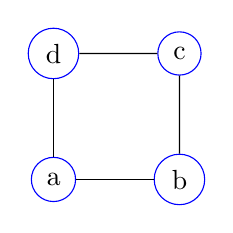
\begin{tikzpicture}
    [scale = .8, auto=center, every node/.style = {circle,draw = blue}]
    \node (n1) at (0,0) {a};
    \node (n2) at (2,0) {b};
    \node (n3) at (2,2) {c};
    \node (n4) at (0,2) {d};
    \foreach \from/ \to in {n1/n2,n2/n3,n3/n4,n4/n1}
      \draw (\from) -- (\to);
  \end{tikzpicture}
\end{center}

\subsection{a directed graph with 5 vertices and 3 edges?}
assuming you mean arcs by edges since in a digraph, there are no edges.

\begin{center}
  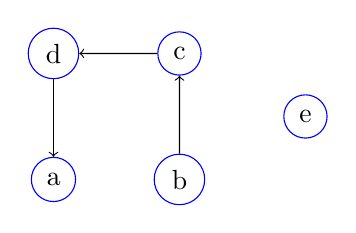
\begin{tikzpicture}
    [scale = .8, auto=center, every node/.style = {circle,draw = blue}]
    \node (n1) at (0,0) {a};
    \node (n2) at (2,0) {b};
    \node (n3) at (2,2) {c};
    \node (n4) at (0,2) {d};
    \node (n5) at (4,1) {e};
    \foreach \from/ \to in {n2/n3,n3/n4,n4/n1}
      \draw[->] (\from) -- (\to);
  \end{tikzpicture}
\end{center}
yes it it possible
\subsection{a disconnected graph (a graph that is not connected) with 5
ices and 7 edges}
no it is not possible, since $K_{4}$ has 6 edges (the maximum amount of edges we can connect with 4 vertices) so we have to connect the 5th node e using our last remaining edge.

\begin{center}
  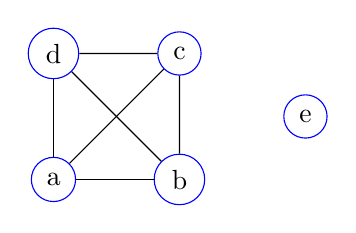
\begin{tikzpicture}
    [scale = .8, auto=center, every node/.style = {circle,draw = blue}]
    \node (n1) at (0,0) {a};
    \node (n2) at (2,0) {b};
    \node (n3) at (2,2) {c};
    \node (n4) at (0,2) {d};
    \node (n5) at (4,1) {e};
    \foreach \from/ \to in {n1/n2,n2/n3,n3/n4,n4/n1,n1/n3,n2/n4}
      \draw (\from) -- (\to);
  \end{tikzpicture}
\end{center}

\subsection{a disconnected, directed graph with 5 vertices and 7 edges }
I assume edges mean arcs (directed edges).
Then yes it is possible since the maximum amount of arcs for $K_{4}$ is 12.\\
So we can completely ignore the 5th node
\begin{center}
  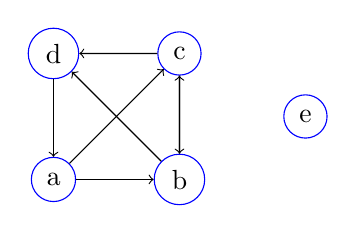
\begin{tikzpicture}
    [scale = .8, auto=center, every node/.style = {circle,draw = blue}]
    \node (n1) at (0,0) {a};
    \node (n2) at (2,0) {b};
    \node (n3) at (2,2) {c};
    \node (n4) at (0,2) {d};
    \node (n5) at (4,1) {e};
    \foreach \from/ \to in {n3/n2,n1/n2,n2/n3,n3/n4,n4/n1,n1/n3,n2/n4}
      \draw[->] (\from) -- (\to);
  \end{tikzpicture}
\end{center}

\subsection{a graph with 3 vertices and 5 edges }
No, since $K_{3}$ has 3 edges and the maximum amount of edges for 3 vertices
is represented by 
  \[ E(K_{3}) = 3\]
\begin{center}
  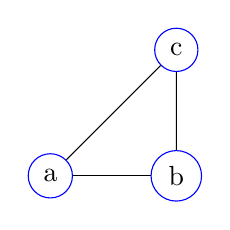
\begin{tikzpicture}
    [scale = .8, auto=center, every node/.style = {circle,draw = blue}]
    \node (n1) at (0,0) {a};
    \node (n2) at (2,0) {b};
    \node (n3) at (2,2) {c};
    \foreach \from/ \to in {n1/n2,n2/n3,n1/n3}
      \draw (\from) -- (\to);
  \end{tikzpicture}
\end{center}
we can't fit 5 edges between 3 vertices.
\subsection{a directed graph with 3 vertices and 5 edges}
I assume that by edges, we are meaning arcs.
then yes it is possible since the maximum amount of arcs for 3 vertices is 6
\begin{center}
  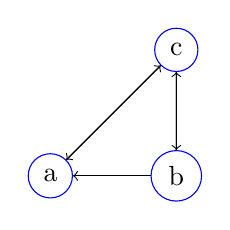
\begin{tikzpicture}
    [scale = .8, auto=center, every node/.style = {circle,draw = blue}]
    \node (n1) at (0,0) {a};
    \node (n2) at (2,0) {b};
    \node (n3) at (2,2) {c};
    \foreach \from/ \to in {n2/n3,n1/n3,n2/n1,n3/n2,n3/n1}
      \draw[->] (\from) -- (\to);
  \end{tikzpicture}
\end{center}

\section{Given a Graph} Given the following graph:

\begin{center}
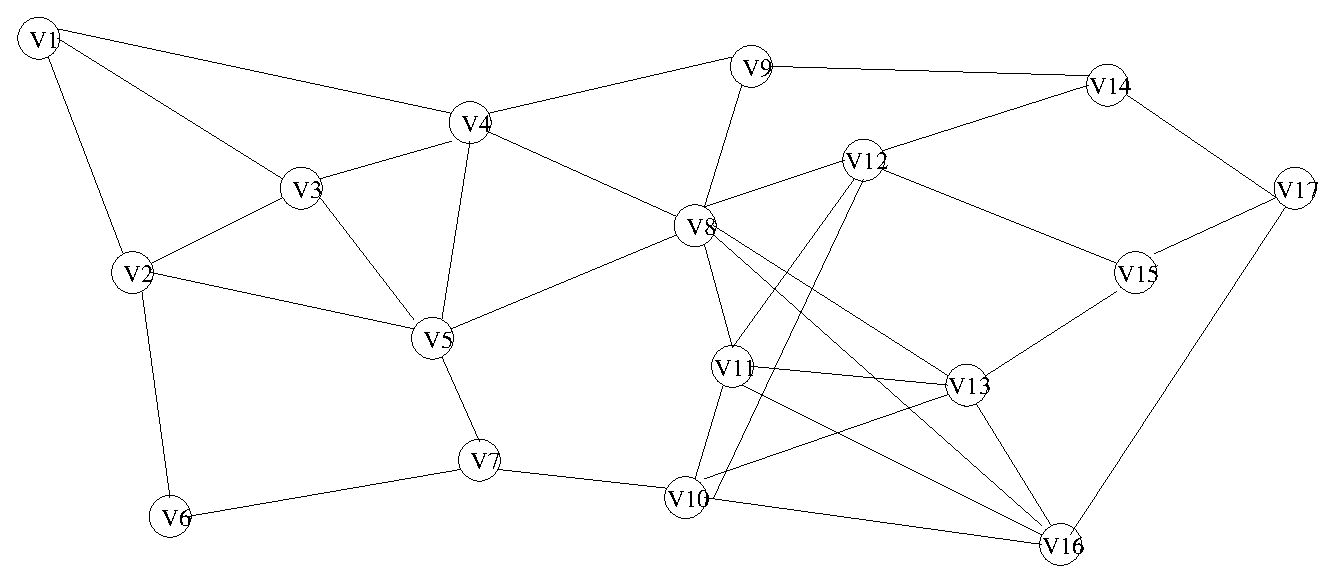
\includegraphics[scale=0.7]{graph.eps}
\end{center}

\subsection{Is this graph connected?}
Yes it is complete, since I can go from any node to any other node.
\subsection{Is this graph complete?  Why/Why not?}
No, there is no edge between V1 and V6.\\
However, there exists a subgraph $K_{4}$
\subsection{What is the minimum degree of the graph?}
minimum degree is 2, on node V6
\subsection{What is the maximum degree of the graph?}
maximum degree is 7, on node V8
\subsection{What is the largest clique in the graph?}
\[K_{4}\] \[V8,V11,V16,V13\]

\subsection{Is the graph planar? Why/Why not?}
No, there exists a subgraph $K_{4}$ $V8,V11,V16,V13$ inside.\\
We know that $K_{4}$ is non-planar.\\
\subsection{What is the shortest path from V1 to V17? How long is it?}

\[V1\rightarrow V4\rightarrow V8\rightarrow V16\rightarrow V17\]
it is length 4
\subsection{What is the longest path from V1 to V17?  How long is it?}
\[V1\rightarrow V4 \rightarrow V9 \rightarrow V14 \rightarrow V12 \rightarrow\]
\[V15 \rightarrow V13 \rightarrow V10 \rightarrow V7 \rightarrow\]
\[V6 \rightarrow V2\rightarrow V3\rightarrow V5 \rightarrow\]
\[V8 \rightarrow V11\rightarrow V16\rightarrow V17 \]
length of 16. All the vertices are visited exactly once
\end{document}
